\documentclass[12pt]{article}
\usepackage{tabularx}
\usepackage{graphicx} % Required for inserting images
\usepackage{dirtytalk}
\usepackage{pgfplotstable} 
\usepackage{pgfplots}
\usepackage{datatool}
\usepackage{siunitx}
\usepackage[hyphens]{url}  % Allows line breaks at hyphens
\usepackage{hyperref}
\usepackage{dirtytalk}
\usepackage{graphicx}
\usepackage{microtype}
\usepackage[backend=biber, defernumbers=true]{biblatex}

\hypersetup{
    colorlinks=true,
    linkcolor=blue,
    filecolor=blue,      
    urlcolor=blue,
    citecolor=blue,
}

% Define categories for all 4 of us, add your SOURCE NAME to YOUR CATEGORY, and store sources in MAIN.BIB:
\DeclareBibliographyCategory{casper}
\DeclareBibliographyCategory{joar}
\DeclareBibliographyCategory{nicole}
\DeclareBibliographyCategory{zongkai}
\addtocategory{casper}{frey2017future, felten2019occupational, riedl2015using, katz2017general, esteva2017dermatologist}
\addtocategory{joar}{AIWorries, IntelligenceExplosion, MyanmarCleansing}
\addtocategory{nicole}{johnson1985technology, russell2015research}
\addtocategory{zongkai}{realriskofai, futuremployment}
\addbibresource{main.bib} % Import sources

\pgfplotsset{compat=1.18}

\begin{document}

\begin{titlepage}
    \centering
    \vspace*{60pt}
    \Huge
    \textbf{Artificial Intelligence Essay \\ DD2380}\\
    \vspace{30pt}
    \Large
    \textbf{Group Number:} 46\\
    \vspace{10pt}
    \large
    \textbf{Group Members:}\\
    \vspace{10pt}
    Casper Kristiansson (casperkr@kth.se)\\
    Nicole Wijkman (nwijkman@kth.se)\\
    Zongkai Zhang (zongkai@kth.se)\\
    Joar Gunnarsson (joargu@kth.se)\\
    \vfill
    \large
    \today
\end{titlepage}


\newpage
\begin{center}
    \huge
    \textbf{Individual Essays}
\end{center}

\section{Casper Kristiansson (casperkr@kth.se)}
{
\setlength\parindent{0pt}   % Disable paragraph indent.
\setlength{\parskip}{\bigskipamount}    %Newline after each paragraph
Throughout history, technological advances have been phasing out and rendering certain skills to become obsolete. Over the past 2 decades, the increased usage of personal computing and the internet have revolutionized the workforce creating a decline in traditional roles. Simultaneously this shift has triggered the emergence of entirely new industries \cite{frey2017future}.

Recent technological advances, particularly in computing and AI have resulted in labor market polarization. As stated in the paper "The Occupational Impact of Artificial Intelligence: Labor, Skills, and Polarization" by Felten, Reaj, and Seamans \cite{felten2019occupational}, \say{This can lead to labor market polarization, where middle-skill, middle-income jobs are negatively affected by innovation, while low and high-skill occupations continue to grow.} Consequently, middle-income jobs face decreased job security due to higher automation risks. This polarization widens the gap between needed and existing labor force skills. Society must adapt to the changes in the job market structure due to both jobs and industries becoming obsolete.

Artificial intelligence has truly already revolutionized the job market, especially significantly impacting cognitive tasks. Many cognitive tasks that were once considered only humans performed are now being automated. AI's capability in cognitive tasks predicts a shift in the job market. It has been shown that AI has improved the efficiency and performance of cognitive tasks in areas like legal research and proceedings \cite{katz2017general}, as well as medical diagnostics \cite{esteva2017dermatologist}. Despite skepticism, AI can execute cognitive tasks, like decision-making, raising ethical concerns about transparency and fairness.

While AI continues to grow leads to an increase in the jobs where it is required to collaborate between a human and an AI. As technology usage increases (especially AI) will lead to the labor market needing to possess more skills. Proficiency in digital skills will become a fundamental requirement for the workforce, not only in the operation of technology but also in understanding the consequences of it.

While AI does provide transparency, accountability, and fairness it has been shown that teaching human values to an artificial agent can reverse engineer cultural values. While this does have potential benefits it does also provide potential drawbacks \cite{riedl2015using}. Providing cultural understanding enables AI to understand human cultures and societal norms which can provide improvements in interactions with it. However, implications such as biases and stereotypes in AI cause ethical dilemmas. Understanding human values is more complex than one might think especially in the rapid cultural changes where AI might not be up-to-date with the current values and societal norms.

The integration of AI in the workplace led to the evolution of the education program. As machines take over routine tasks there is an increased need for workers with advanced technical and analytical skills. This has led to the growth and development of the concept of lifelong learning, where humans have to continuously learn new skills and improve them to stay relevant in their field.

This raises an interesting question, do humans now compete with AI? With AI systems capable of operating 24/7 how can a normal worker compete with it? While introducing competitiveness in various fields and industries can be positive, it raises the question of its impact on an individual's work-life balance. Situations like these result in a reevaluation of work norms. While AI and computing in general have caused a lot of industries, fields, and jobs to die out it has also introduced a lot of new ones. This shift challenges us to redefine our understanding of work, productivity, learning, and value in an AI-centered world. Ultimately, the key may lie in understanding AI's capabilities with human creativity and compassion, creating a future where technology complements rather than competes with human labor.

Word count: 596 words.

}

\printbibliography[title={References - Casper}, category=casper]



\section{Joar Gunnarsson (joargu@kth.se)}
{
\setlength\parindent{0pt}   % Disable paragraph indent.
\setlength{\parskip}{\bigskipamount}    %Newline after each paragraph
One worry regarding AI is how good it is at manipulating human behaviour while being very scalable. One example of this is social media algorithms, which determine the content shown on the site. These applications collect a huge amount of data about what the users, which can then be used to create a detailed user profile. This, together with control of the content, makes it possible for AI algorithms to influence human behaviour by modifying what a user is exposed to. As AI becomes smarter and better, social media algorithms will become more able to influence human behaviour, but it is already happening today \cite{AIWorries}.

Personally, I agree that this is a reason to worry.A big part of how we consume news and information is via these social media apps, such as Facebook. One example I found of Facebook's algorithms influencing human behaviour is the ethnic cleansing in Myanmar in 2017, that targeted a minority group in Myanmar, the ``Rohingya''. The algorithms used by Facebook exacerbated the hostility against this group, which in turn had real world consequences on human behaviour \cite{MyanmarCleansing}. This could become an even larger problem in the future. If the company in charge of the AI algorithm was a malicious actor, the harm could be even greater. 

While there are risks with using AI, AI can also be essential to curate the content that is shown to the users. More and more content is created every day, and the user is not interested in everything. However, it is important that the control of what is shown comes from the user, and is tuned to what content they want to see, and not from someone else that wants to control the users opinions \cite{AIWorries}.

A second thing that many people are worried about is the so called \textbf{AI singularity}. This is a phenomenon where if we create an general artificial intelligence that is smarter than us, this AI will be able to create an AI which is smarter than itself. This would then continue indefinitely, resulting in AI so much smarter than humans that human intelligence becomes obsolete \cite{IntelligenceExplosion}.

There are some who criticize this idea. The article ``The implausibility of intelligence explosion'' present some counter-arguments. The author of the article posits that this idea is built upon a misunderstanding of intelligence. One such supposed misunderstanding is that \textit{general intelligence} does not, in fact, exist. For example, human intelligence is specialized in a certain task, namely the task of being human. Furthermore, it is possible that human intelligence is only possible in a human environment. Humans raised by wild animals are very rarely able to function in our society \cite{IntelligenceExplosion}. While this might be the case, I don't think this excludes the possibility of an AI explosion. Even if general intelligence is impossible, it might still be possible for an AI to develop extremely high ``human'' intelligence. Also, if the environment is vital for the development of intelligence, a computer could simulate this.

The author also makes the argument that even if AI improves itself recursively, it be a non-explosive linear one. One example he mentions is personal investing. The more money you have, the more money the investments can earn. And usually, this results in linear growth, since as the savings increase, so does the spending, for an average human \cite{IntelligenceExplosion}. However, this is a very unconvincing example. In fact, personal spending is a very good example of the opposite; it is a recursive improvement that very easily can lead to explosive growth.

Word count: 581 words.
}

\printbibliography[title={References - Joar}, category=joar]



\section{Nicole Wijkman (nwijkman@kth.se)}
{
\setlength\parindent{0pt}   % Disable paragraph indent.
\setlength{\parskip}{\bigskipamount}    %Newline after each paragraph

%Reflect on your reading: What are the most important take-aways regarding ethical and societal aspects of AI from the read material? Do you agree or disagree with them? 

%Write an essay (500-600 words excluding references) where your summarize your reflection on the reading. Your text must:

%- discuss and reflect on current ethical and societal aspects of AI, and
%- cite relevant literature where appropriate. Naturally, your essay will have to contain references to at least the 2 chosen papers you read, but feel free to read more and refer to more sources.

In recent years there has been a rapid advancement of artificial intelligence (AI) technologies, and as a result, the ethical and social aspects of AI are more relevant than ever. As with any new technology, it is important that there is a concern regarding the impact of AI on both individuals and society as a whole. 

Personally, I think one of the most important takeaways from both selected papers is that there is a necessity for a robust ethical framework for AI. The paper \say{Technology with No Human Responsibility} by Deborah G. Johnson truly highlights the need for ethical regulations and considerations when it comes to AI development \cite{johnson1985technology}. According to Johnson, AI algorithms can exhibit biases, discriminate, and invade privacy. As these types of algorithms are increasingly integrated into our daily lives, they have the potential to be dangerous without proper regulations.

Johnson underscores that AI systems that AI systems can inadvertently perpetuate biases that are present in their training data, which reinforces existing inequalities. She draws attention to cases where AI algorithms used in hiring processes can discriminate against specific demographic groups due to biases in historical hiring data. This not only harms individuals but also perpetuates societal disparities and is a direct consequence of neglecting ethical responsibility in AI development.

I wholeheartedly agree with Johnson's emphasis on the importance of ethics in AI development. Considering how AI algorithms are trained on data created by humans, who are part of a society full of disparities, ethical considerations have to be embedded into the very fabric of AI design and deployment; they cannot come secondary. I believe that adopting ethical AI principles, like fairness and accountability, is crucial to ensure that AI benefits society rather than harms it. 

Moreover, the paper \say{Research Priorities for Robust and Beneficial Artificial Intelligence} by Stuart Russell, Daniel Dewey, and Max Tegmark, highlights the significance of building trust in AI systems\cite{russell2015research}. They emphasize the need for AI developers to act responsibly and prioritize the safety of society. This goes hand-in-hand with the paper by Johnson, which emphasizes the importance of building trustworthy AI systems that respect human values.

Rusell, Dewey, and Tegmark discuss the development of autonomous vehicles. They point out that ensuring these vehicles operate safely and reliably is a very important ethical concern. Without very rigorous testing and safety measures, the consequences of failures would be catastrophic, both for individuals and society at large. This further exemplifies the need for a deep sense of responsibility and care in AI development, especially in scenarios where human lives are at stake.

I agree with the authors that there is great significance in trust. It is an essential aspect of the widespread adoption of AI. I believe developers of AI algorithms have a moral responsibility to ensure that the development and deployment of AI systems are safe and trustworthy. This includes thorough testing, ethical sourcing of training material, and addressing potential biases.

Conclusively, these papers both offer valuable insights into both ethical and societal aspects of AI. They underscore the importance of ethical frameworks, as well as addressing biases and building trust in AI systems. These papers made it very clear to me that to fully realize the benefits of AI for society, ethical considerations must be placed at the forefront of AI development.

Word count: 551 words.
}


\printbibliography[title={References - Nicole}, category=nicole]



\section{Zongkai Zhang (zongkai@kth.se)}
{
\setlength\parindent{0pt}   % Disable paragraph indent.
\setlength{\parskip}{\bigskipamount}    %Newline after each paragraph

% essay goes here
Artificial Intelligence is changing how we live and work, and it's important to consider its ethical use and impact on society. The article "The Real Risks of Artificial Intelligence" challenges us to consider the reliability and ethical implications of AI. David Parnas presents several historical examples from the early days of AI research to highlight potential issues with current AI applications. He criticizes the vague use of the term AI and suggests that without a solid scientific foundation, AI systems can be unpredictable and potentially dangerous \cite{realriskofai}.

In the paper "The Future of Employment", the author gives a rigorous analysis suggesting a significant portion of jobs could be automated, raising concerns about job security for many. The paper's findings are a wake-up call to the reality that AI and automation could lead to substantial job losses, especially in roles that do not require advanced education \cite{futuremployment}. This potential shift in the job market calls for serious reflection on how we can prepare for a future where many traditional jobs may no longer exist.

Both articles suggest that we need to create AI responsibly. AI should be made with clear rules that everyone understands and follows. It should be safe, fair, and help society, not just make money for a few people. The future of work is changing because of AI, and we must make sure that education and job training programs keep up with these changes. This way, people can learn new skills that are needed for the kinds of jobs that will be available in the future.

From my perspective, building AI responsibly means developing technology that is trustworthy, and works for the common good. It's not just about creating smart machines but about ensuring these machines operate within ethical boundaries. Policymakers, educators, and AI developers must come together to address these challenges. Education systems need to adapt, providing training that aligns with the future job market, and policies must be in place to support those impacted by technological displacement.

Furthermore, the ethical deployment of AI requires a keen focus on minimizing societal harm. AI holds the potential to deepen existing inequalities if not guided by ethical principles. As such, the development of AI should be done with a commitment to fairness, aiming to reduce the divide between different societal groups.

The societal implications of AI's rise are vast. Beyond job displacement, AI could change the nature of work itself, requiring a rethinking of job functions, economic models, and the definition of work. The prospect of AI systems performing tasks that were once thought to be uniquely human challenges our understanding of human value in the workforce. As AI becomes more popular in our lives, we must also consider its impact on social interactions and individual privacy. It's crucial to establish boundaries for AI's reach into our private lives and ensure that data usage aligns with ethical standards.

In summary, the occurrence of AI is not just a technical advancement, but also a moment that calls for careful ethical consideration and proper societal planning. While AI offers remarkable opportunities for advancement, it also presents risks that must be managed thoughtfully. The potential for unemployment and increased inequality necessitates a comprehensive response that includes updated educational programs, support for displaced workers, and ethical guidelines for AI development. It is our collective responsibility to steer AI in a direction that keep human dignity, promotes societal welfare, and ensures that the benefits of AI innovations are shared equally across society.


Word count: 579 words. % fill in number of words at the x

}

\printbibliography[title={References - Zongkai}, category=zongkai]


\newpage
\begin{center}
    \huge
    \textbf{Summary}
\end{center}
\setlength\parindent{0pt}   % Disable paragraph indent.
\setlength{\parskip}{\bigskipamount}    %Newline after each paragraph
{

% Casper
The first essay by Casper Kristiansson was centered around how AI affects and polarizes the labor market. The essay introduces the key word of polarization where AI affects mostly the middle-income jobs where cognitive tasks are extremely popular. While AI probably right now or in the future can replace a lot of low-income jobs like berries picking it is still not worth doing due to multiple aspects like effort and cost. While we know that AI already is replacing a lot of cognitive tasks like legal research can we truly trust AI? We believe that in the current state of AI, we wouldn’t trust AI enough to make important discussions (for example replacing a human doctor). But in the future, we think that we as humans would trust AI more than other humans to make important discussions.

% Joar
The second essay discussed how AI can manipulate human behaviour, and the possibility of an AI explosion. We agreed on how scary it is that AI can influence people so easily using social media. For example, to gradually influence your opinion, the algorithm can slowly introduce things you might not agree with. This is especially concerning for young people, since their brains are not fully developed yet. We also discussed a YouTube experiment, where a brand new account was created and they wanted to see how long it took for the algorithm to start suggesting far-right political videos. After clicking a single joke video containing anti-feminist jokes, the content quickly got more and more extreme. What's scary about this is you might not even notice that it is happening. Is the video just popular, or if was recommended to you to influence your opinion?


% Nicole

The third essay by Nicole Wijkman centered on the ethical aspects of AI and its potential effect on society. The essay discussed potential biases in AI, as well as the need for developers to prioritize the safety of society. The group agreed that there is an important ethical aspect to consider and discussed how AI algorithms need to be transparent with clear regulations to understand the results. We brought up how chatGPT sometimes makes information up based on the dataset it has been trained on, and how this potential spread of false information could be dangerous. The group also discussed the importance of AI being implemented into our society in a responsible manner early on in its development. An example we brought up is if the world became prone to accidents involving AI-driven cars, these might be completely outlawed thus hindering the development in this area. 

%- Generally with AI there is an important ethical aspect. It has to be transparent. Regulations are important, especially when working with AI in cars etc. 
%- Especially now at the start of AI where we don't know how to implement it. if we do it wrong - maybe we have to outlaw automatic cars because people died, even if we create very good algorithms. Also important it doesn't inherit our biases.
%- like with chatgpt, if all schools used chatgpt all of a sudden without teachers then it'd suck.


% Zongkai

The fourth essay also talks about the ethics and responsibilities of AI and here we come up with new thoughts and questions. We think what should we bear in mind is not just AI itself, but also the other human beings who may use AI or may be influenced by the coming up of AI. The question is: Will the world become better if every one use AI in their daily study or work? Will human be more or less intelligent with Artificial Intelligence? We think the answer depends. For educated people or experienced engineers, they may improve their work or generate new ideas with the help of AI. But factory workers or young students, they may also be faced with unemployment or becoming too dependent on AI. Therefore, we think AI should serve different people in different ways. AI is not just more powerful the better, but is more helpful for people the better. 

}
\newpage
\begin{center}
    \huge
    \textbf{Group Picture}
\end{center}

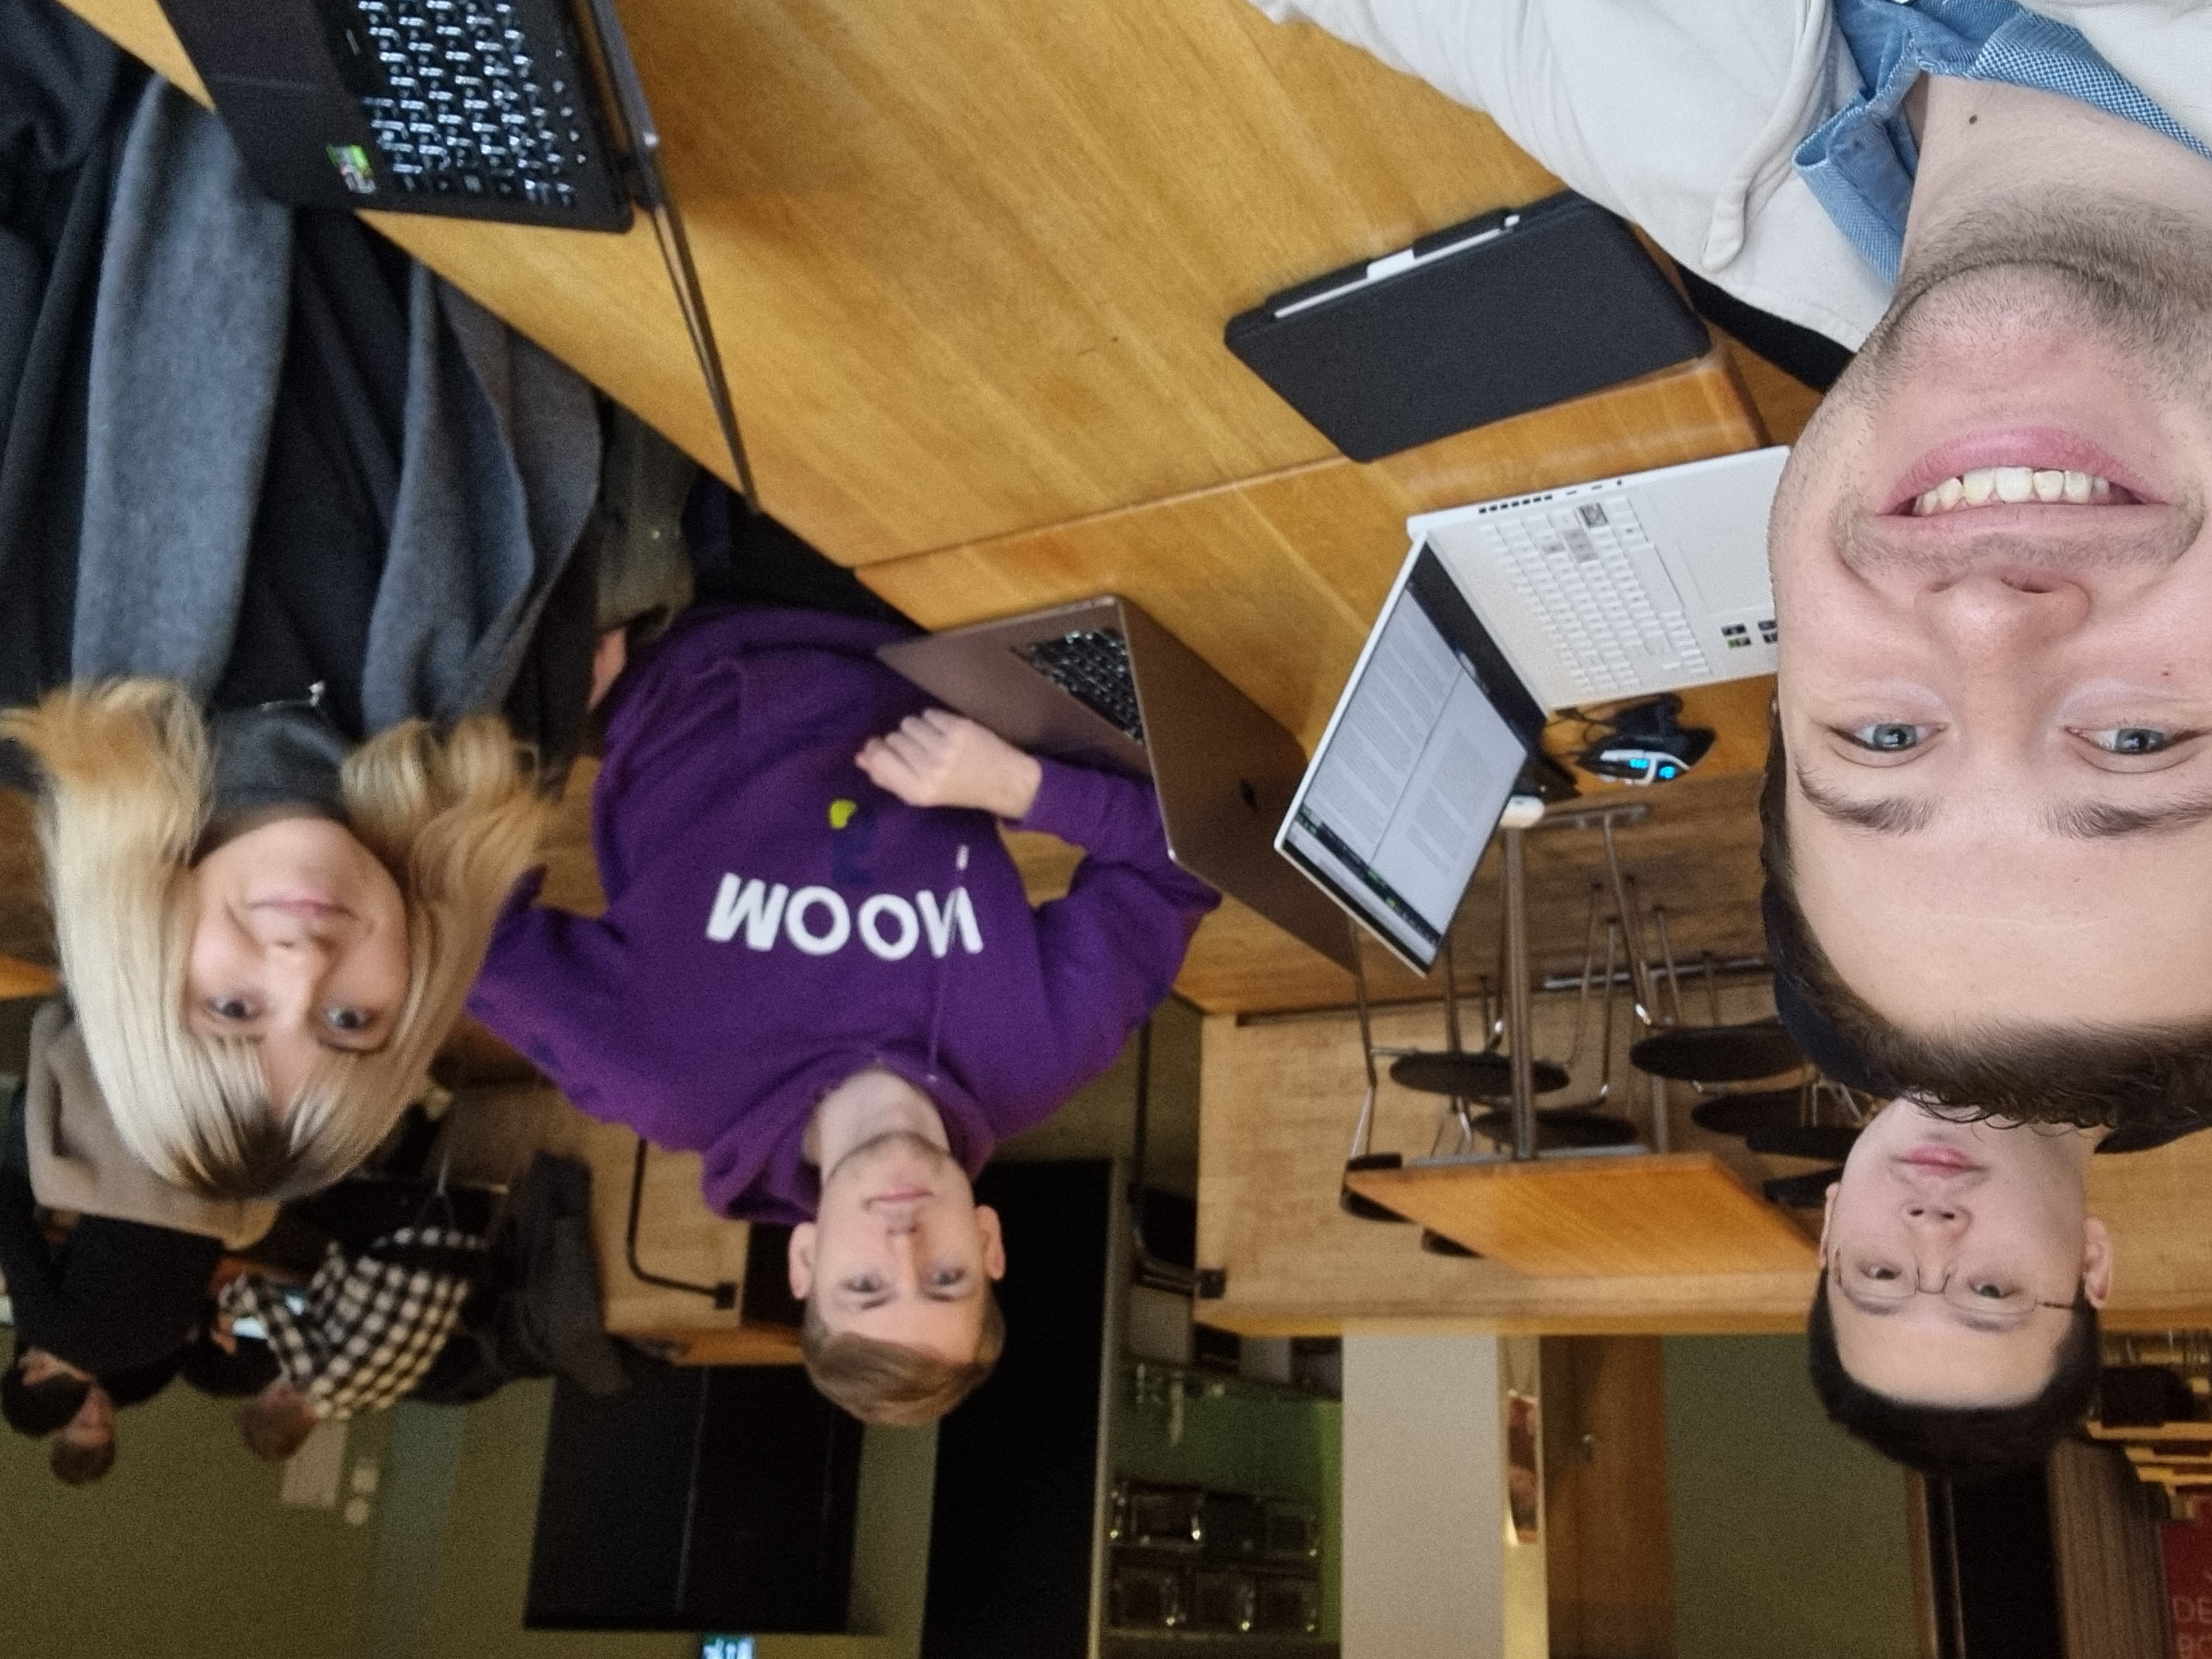
\includegraphics[width=\textwidth, angle=180]{group.jpg}


\newpage

\end{document}
